\chapter{User Interface Design}


This section presents screenshots of the Students and Companies app, highlighting its interface and key features, giving a clear view of how users interact with the platform.

\begin{figure}[H]
    \centering
    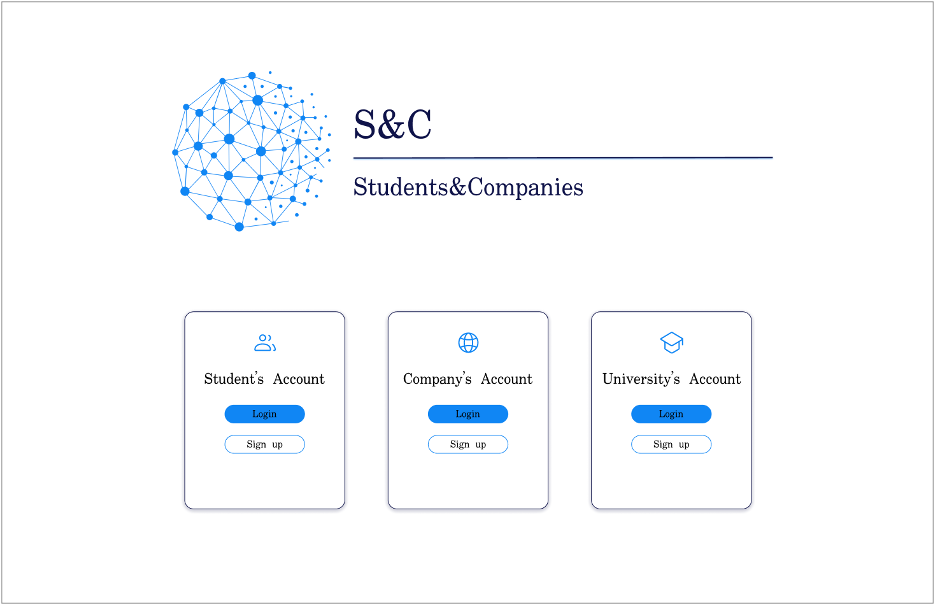
\includegraphics[width=1\linewidth]{DD//Images/UI photos/Home.png}
    \caption{Login Page}
\end{figure}

The Login Page allows users to choose whether to create a new account or log into an existing one. Users can select their role (student, company, or university) to access the appropriate features of the app.

\begin{figure}[H]
    \centering
    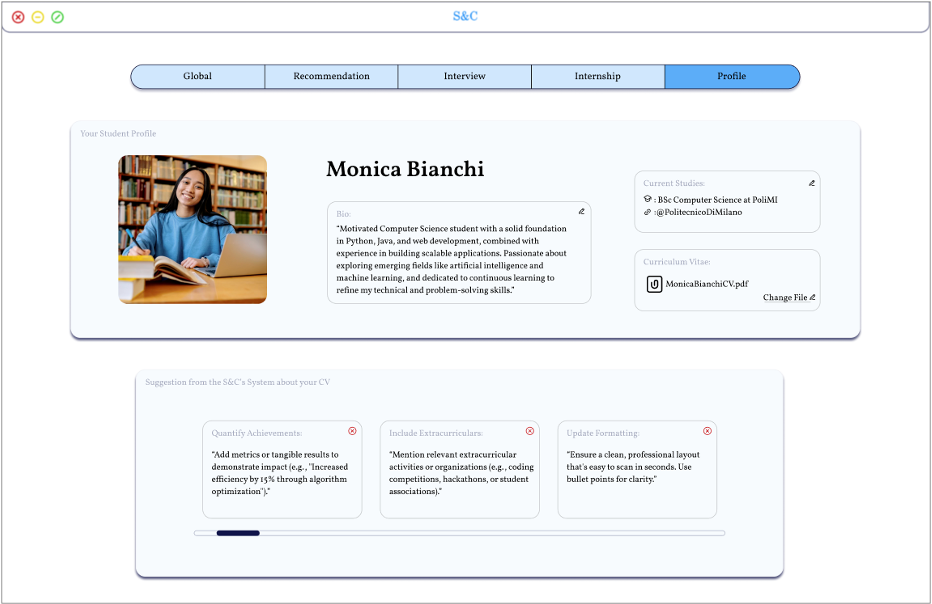
\includegraphics[width=1\linewidth]{DD//Images/UI photos/Student's Profile.png}
    \caption{Student's Profile Page}
\end{figure}

The Student's Profile Page displays the student's photo, bio, and education information, with options to view and update this information. It also allows the student to upload, delete, or re-upload their CV. Below the profile details, the page shows personalized suggestions from the Students and Companies system, offering hints to improve their CV.


\begin{figure}[H]
    \centering
    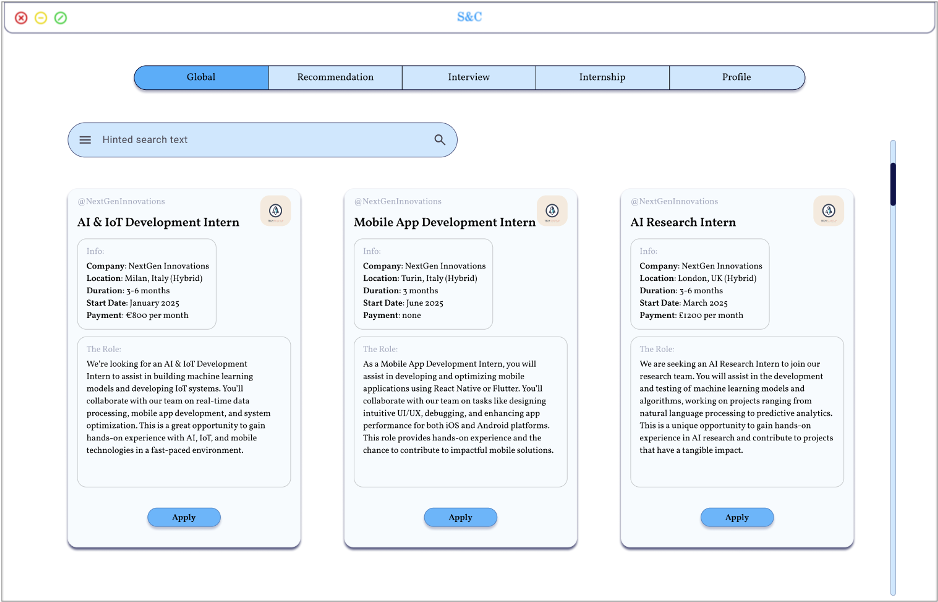
\includegraphics[width=1\linewidth]{DD//Images/UI photos/Student's Global.png}
    \caption{Student's Global Searching Page}
\end{figure}

The Student's Global Searching Page allows students to browse all available internship project descriptions. They can proactively search for internships that match their interests and skills, using keywords or specific parameters. Students also have the option to apply directly to internships that suit them best.

\begin{figure}[H]
    \centering
    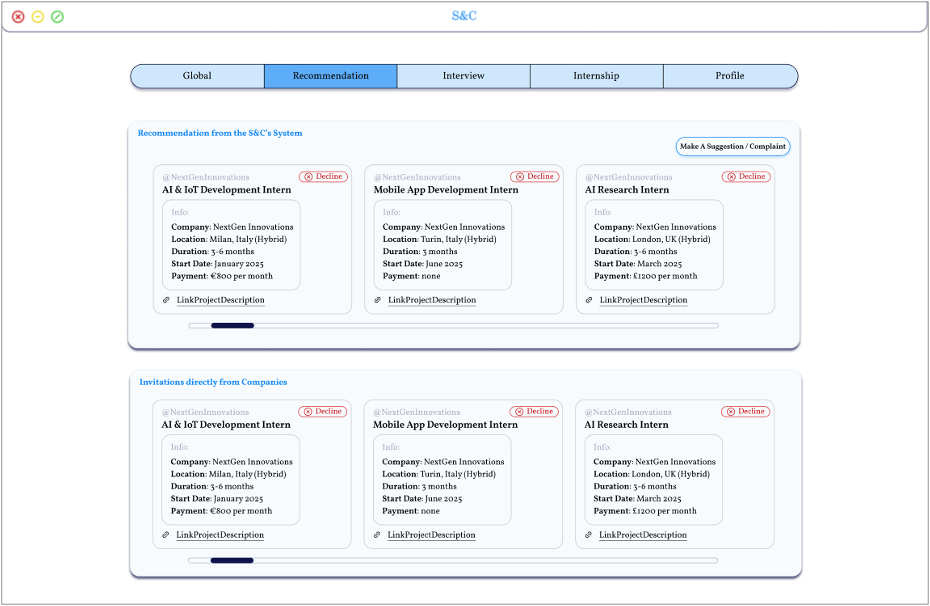
\includegraphics[width=1\linewidth]{DD//Images/UI photos/Student's Recommendations.png}
    \caption{Student's Recommendations Page}
\end{figure}

The Student's Recommendations Page displays internship opportunities suggested by the Students and Companies system, tailored to the student's profile. The student can accepts the recommendation applying for the position. Below these recommendations, the student can also view invitations sent directly from companies. In both cases, the student can apply directly to the internships.

\begin{figure}[H]
    \centering
    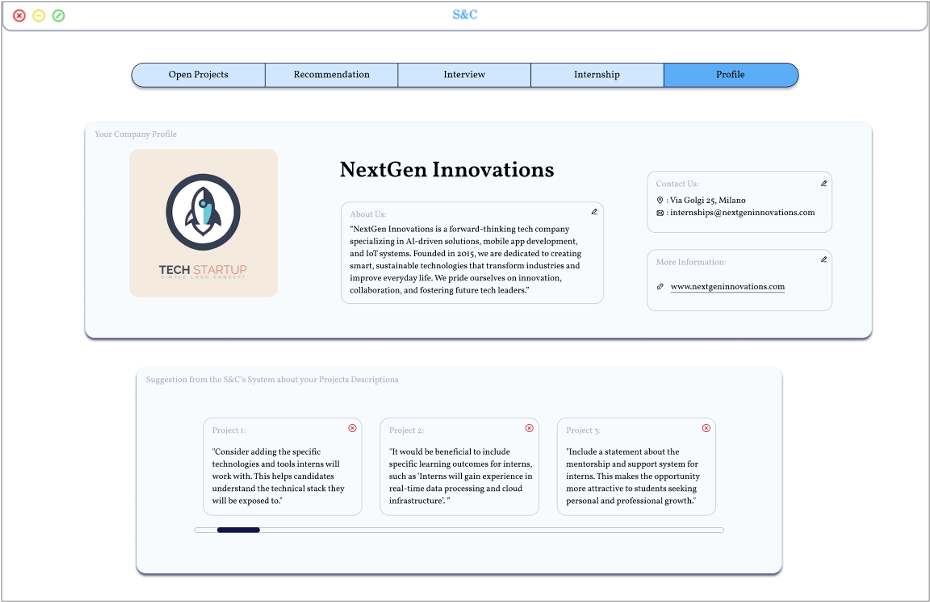
\includegraphics[width=1\linewidth]{DD//Images/UI photos/Company's Profile.png}
    \caption{Company's Profile Page}
\end{figure}

The Company's Profile Page displays the company's bio and all the information they’ve provided about themselves, with the option to edit and update this content. Below, the page shows suggestions from the Students and Companies system on how to improve the descriptions of each posted internship project, making them more appealing and informative.

\begin{figure}[H]
    \centering
    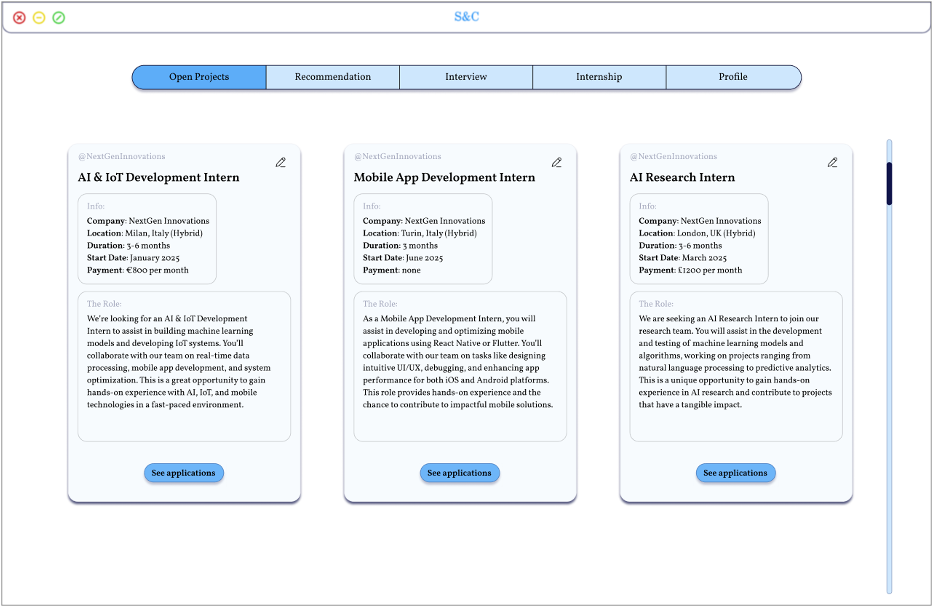
\includegraphics[width=1\linewidth]{DD//Images/UI photos/Company's Projects.png}
    \caption{Company's open projects Page}
\end{figure}

The Company's Open Projects Page displays all the internship project descriptions that the company has published. It offers the option to modify these descriptions and provides direct links to view the applications received for each internship.

\begin{figure}[H]
    \centering
    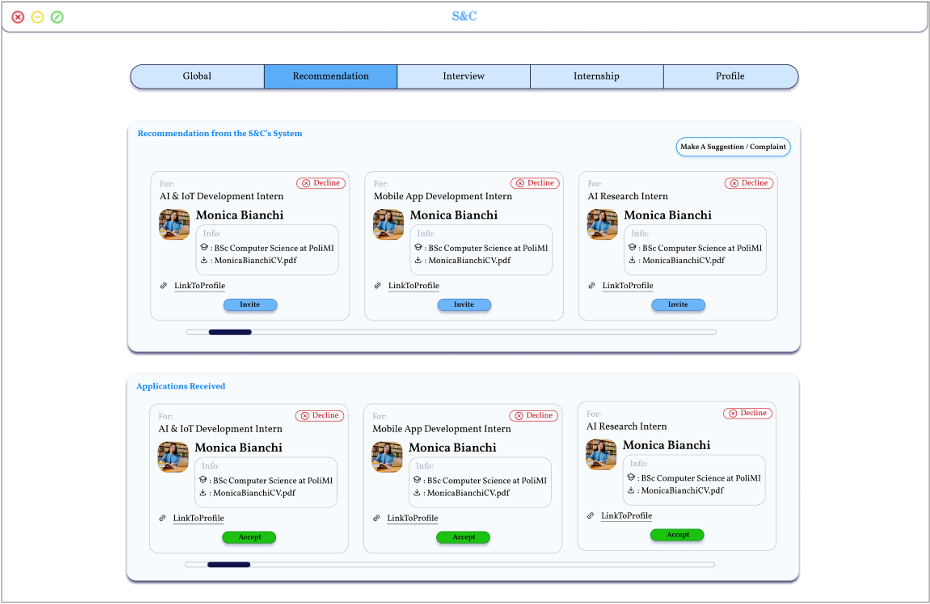
\includegraphics[width=1\linewidth]{DD//Images/UI photos/Company's reccomendations.png}
    \caption{Company's Recommendations Page}
\end{figure}

The Company's Recommendations Page displays a list of recommended candidates from the system, providing a preview of their profiles with a direct link to view more details. The company can accept recommendations and invite students to apply. Below the recommendations, the page also shows all the applications the company has received from students.

\begin{figure}[H]
    \centering
    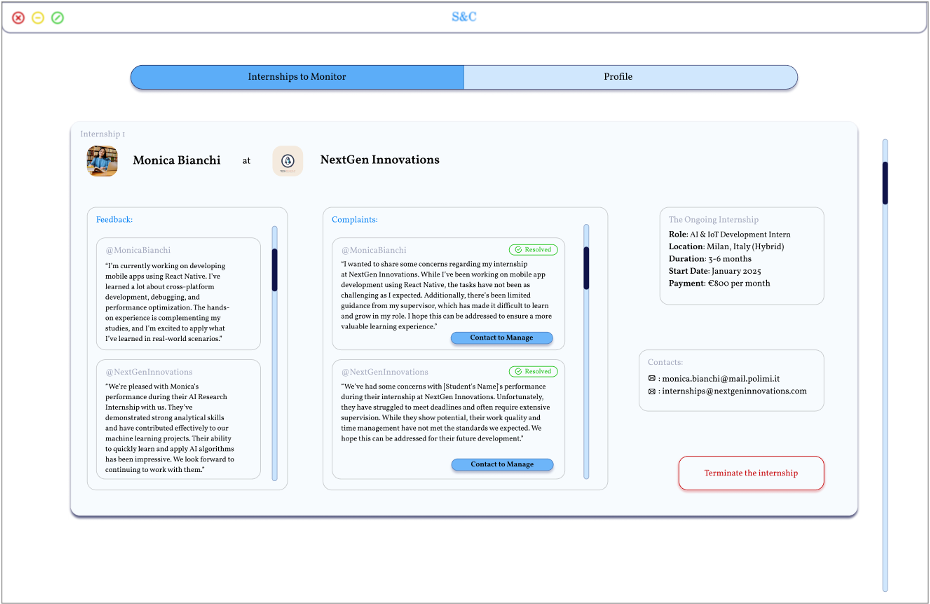
\includegraphics[width=1\linewidth]{DD//Images/UI photos/Universities Monitoring.png}
    \caption{University's ongoing internship Monitoring Page}
\end{figure}

The University's Ongoing Internship Monitoring Page provides a comprehensive overview of all ongoing internships, including details about the student, company, role, and relevant contact information. The page features sections for both feedback and complaints, which can be submitted by either the student or the company. Complaints can be managed within the app or resolved externally, with the option to report the resolution back on the platform.